\chapter{Experiments}
    \section{Preliminary ignition experiments} \label{sec:ignitiontest}
        Once the necessary components of the experiment were integrated, a preliminary testing campaign began to attempt to ignite LSP. The hope was to resolve any unforeseen practical issues, then quickly move on to replicating the power threshold experiments of past LSP literature~\cite{zimakovInteractionNearIRLaser2016,matsuiGeneratingConditionsArgon2019,luCharacteristicDiagnosticsLaserStabilized2022}. The test campaign aimed to answer two questions:
        \begin{itemize}
            \item Can LSP be achieved with this experimental setup at all?
            \item How reliable is LSP ignition with this system?
        \end{itemize}
        To answer this, experimental trials would be run in conditions most favorable to steady LSP formation, i.e. at maximum laser power and maximum test section pressure: \qty{3}{kW} and \qty{20}{bar}. Successful ignition would be determined based on two independent measures:
        \begin{enumerate}
            \item The high-speed camera should be able to image the LSP growing and propagating towards the laser source over the course of the laser pulse, as consistently documented in LSP literature.
            \item A measurable drop in laser energy reaching the Gentec power meter should be observed.
        \end{enumerate}
        LSP would only be deemed to have successfully ignited if the expected behavior was observed with both instruments.

        Laser alignment was immediately found to be a non-trivial problem. In order to successfully ignite the LSP, the laser must be focused onto the arc generated by the spark igniter. To maximize the chance of ignition, the laser flux at the arc must be as high as possible, so the focused laser dot must be as small as possible. This makes alignment tolerances much stricter, as the laser is less likely to be incident on the thin arc at all.

        Compounding this issue was the fact that the path taken by the arc between both electrode tips was not consistent. As seen in \autoref{fig:sparkAlignment}, the location of the arc was highly variable: though an average arc path could be determined, the arc could form up to \qty{1}{mm} away. This made it impossible to ensure consistent alignment between the arc and the laser focus. This issue could be alleviated by repeatedly triggering the spark, but the smart coil had a nominal delay of \qty{3}{ms} between sparks, only allowing up to three ignition attempts within a single laser pulses, making this approach of little viability for high-power pulse laser tests. Repeated sparks could be used with CW laser operation at \qty{300}{W}, but the lower laser power also reduces the likelihood of successful LSP ignition.

        \begin{figure}[h]
            \centering
            \begin{subfigure}[t]{0.47\textwidth}
                \centering
                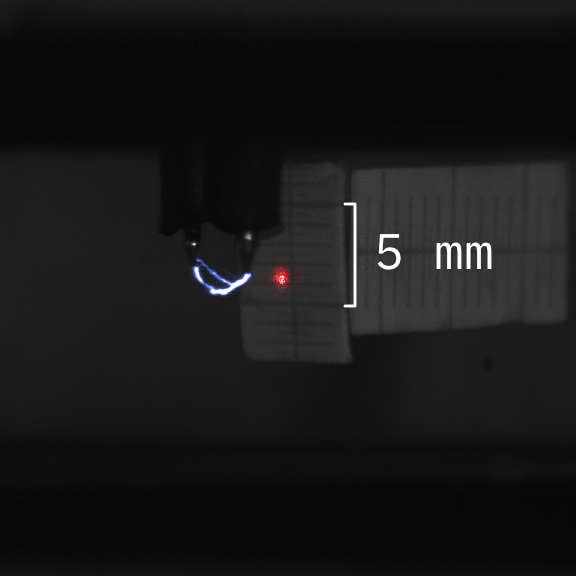
\includegraphics[]{assets/3 design/sparkAlignment_one.jpg}
                \caption{Single arc generated by the spark igniter}
                \label{fig:sparkAlignment_one}
            \end{subfigure}
            \hfill
            \begin{subfigure}[t]{0.47\textwidth}
                \centering
                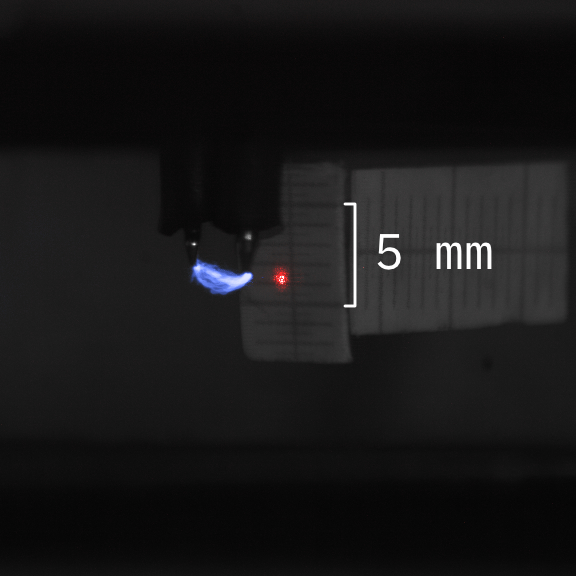
\includegraphics[]{assets/3 design/sparkAlignment.jpg}
                \caption{Several arcs stacked together to create a ``heatmap'' of arc formation. Note the large variance in the path taken by the arc.}
                \label{fig:sparkAlignment_heatmap}
            \end{subfigure}
            \caption[Composite photos made during a typical spark-laser alignment procedure]{Composite photos made during a typical spark-laser alignment procedure. The gray-scale background, blue arcs, and red guide laser photos were taken separately then stacked together to be able to compare the relative position of the arcs and laser.}
            \label{fig:sparkAlignment}
        \end{figure}

        In addition, the laser could not be aligned without placing reflecting or scattering material in the beam path. As seen in \autoref{fig:sparkAlignment}, a target must be placed near the ignition point to perform the alignment (and also serves as a scale indicator). However, this alignment target had to be removed to pressurize the test section, which was required both to determine the spark location, and to perform the LSP ignition test. Pressurization cycles and the placing/removal of this target made the alignment process slow and cumbersome. Alignment with the arcs could not be confirmed visually since the target could not be present when pressurizing the test section.

        Despite these difficulties, several attempts were made to ignite LSP with this method, and a few were successful. The first successful test was performed at \qty{10.02}{bar} with a full power pulse (\qty{30.8}{J}). A paper target had been placed next to the electrodes to facilitate alignment, so no measurements were made of the pulse energy transmitted through the plasma for the first few successful tests. However, high-speed footage showed strong evidence of plasma formation: a bright flash saturating the camera sensor, igniting at the time of spark formation, as seen in \autoref{fig:lsp1}. Such a flash had never been observed in past (failed) ignition tests. Though this suggested that some plasma had been formed, there was a possibility that the alignment target was affecting the experiment and may even have contributed to the ignition. The footage showed evidence of particles being ejected from the area around the ignition point, possibly due to the interaction between the laser, plasma, and the paper target.

        \begin{figure}[h]
            \centering
            \begin{subfigure}[t]{0.32\textwidth}
                \centering
                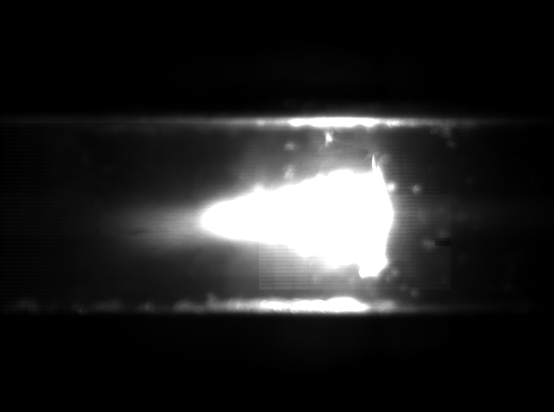
\includegraphics[width=\textwidth]{assets/3 design/LSP1_frames/20.jpg}
                \caption{2.0~ms}
                \label{fig:lsp1_20}
            \end{subfigure}
            \hfill
            \begin{subfigure}[t]{0.32\textwidth}
                \centering
                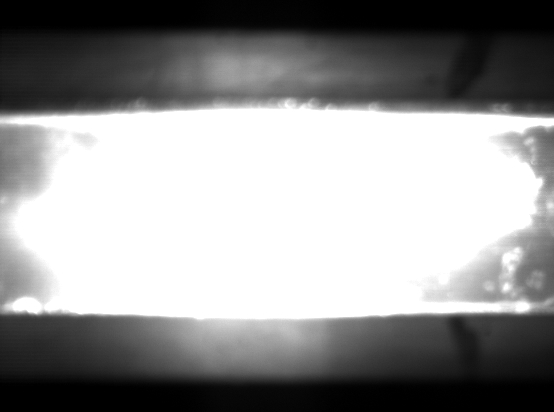
\includegraphics[width=\textwidth]{assets/3 design/LSP1_frames/30.jpg}
                \caption{3.0~ms}
                \label{fig:lsp1_30}
            \end{subfigure}
            \hfill
            \begin{subfigure}[t]{0.32\textwidth}
                \centering
                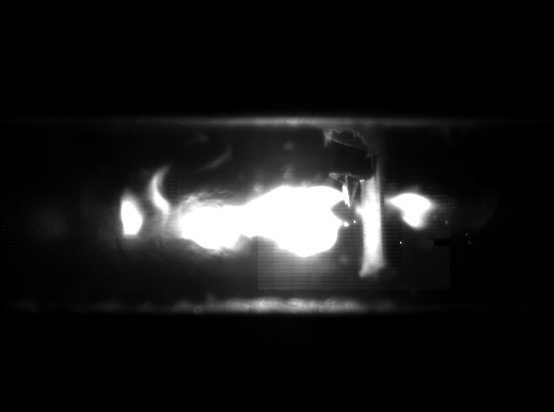
\includegraphics[width=\textwidth]{assets/3 design/LSP1_frames/75.jpg}
                \caption{7.5~ms}
                \label{fig:lsp1_75}
            \end{subfigure}
            \caption{High-speed footage frames of first successful LSP ignition}
            \label{fig:lsp1}
        \end{figure}

        The experiment was repeated with the target several times, ensuring that the flash was not the result of merely burning a hole through the paper target. In addition, the exposure settings were adjusted (increasing the ND filter to ND2048 and setting the aperture to \textit{f}/22) to provide a clearer view of the brightest part of the frame, the LSP core. A snapshot of the resulting footage is shown in \autoref{fig:lsp3}, revealing a slender plasma core, approximately contained within the focused laser beam (note the thinner right tip of the LSP compared to the left tip). The plasma was observed to grow towards the source of the laser, as reported in experimental LSP literature. This appearance and growth behavior provided additional evidence that these tests were truly achieving laser-sustained plasma, as opposed to some other phenomenon.

        \begin{figure}[h]
            \centering
            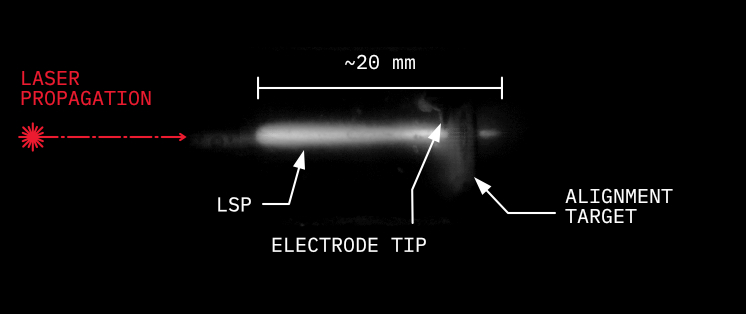
\includegraphics[]{assets/3 design/LSP3_annotated.jpg}
            \caption[Third successful LSP test ignited by arc discharge]{Third successful LSP test ignited by arc discharge. Snapshot from just before the end of the laser pulse. Dimension is approximate.}
            \label{fig:lsp3}
        \end{figure}

        To provide complete confidence that this indeed was LSP, more experiments were performed without the paper target. This allowed the measurement of the laser energy not absorbed by the plasma, and would confirm that the LSP is ignited purely by the spark, as opposed to ablated material from the paper target. 

    \section{Power threshold}
    
    \begin{figure}[h]
    \centering
    \begin{subfigure}[t]{0.3\textwidth}
        \centering
        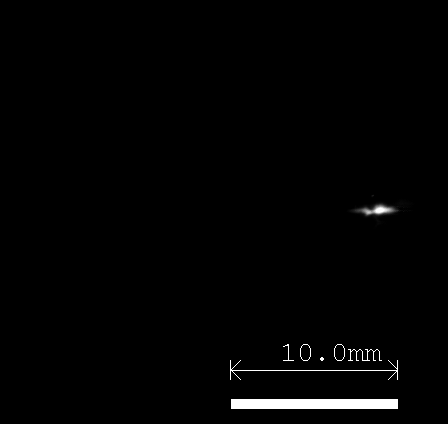
\includegraphics[width=\textwidth]{assets/4 experiments/V1 Spark Ignition Frames/LSP142_SPRK15_Fr32.bmp}
        \caption{\qty{3.2}{ms}}
        %\label{fig:V1_ignition_frames_16}
    \end{subfigure}
    \hfill
    \begin{subfigure}[t]{0.3\textwidth}
        \centering
        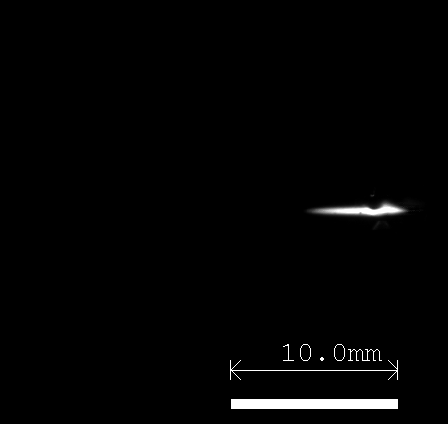
\includegraphics[width=\textwidth]{assets/4 experiments/V1 Spark Ignition Frames/LSP142_SPRK15_Fr33.bmp}
        \caption{\qty{3.3}{ms}}
        %\label{fig:ignition_frames_17}
    \end{subfigure}
    \hfill
    \begin{subfigure}[t]{0.3\textwidth}
        \centering
        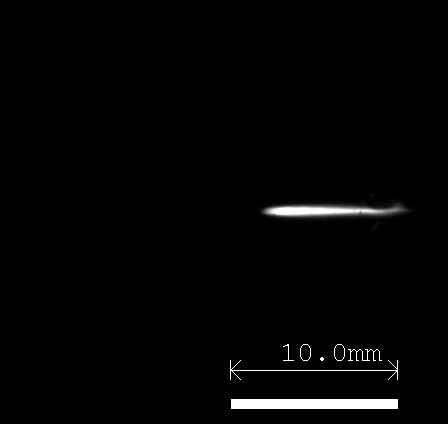
\includegraphics[width=\textwidth]{assets/4 experiments/V1 Spark Ignition Frames/LSP142_SPRK15_Fr35.bmp}
        \caption{\qty{3.5}{ms}}
        %\label{fig:ignition_frames_18}
    \end{subfigure}
    \begin{subfigure}[t]{0.3\textwidth}
        \centering
        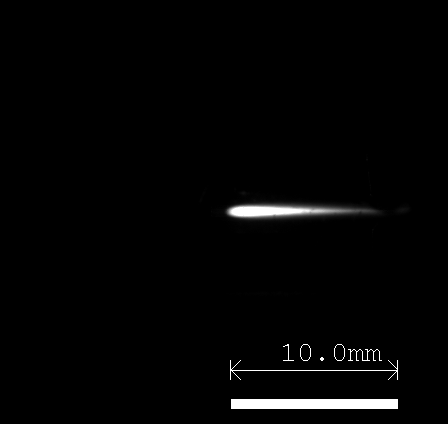
\includegraphics[width=\textwidth]{assets/4 experiments/V1 Spark Ignition Frames/LSP142_SPRK15_Fr38.bmp}
        \caption{\qty{3.8}{ms}}
        %\label{fig:ignition_frames_19}
    \end{subfigure}
    \hfill
    \begin{subfigure}[t]{0.3\textwidth}
        \centering
        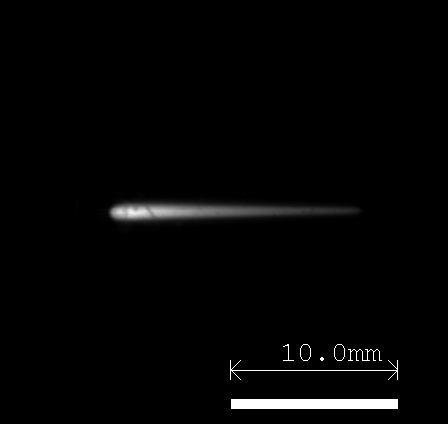
\includegraphics[width=\textwidth]{assets/4 experiments/V1 Spark Ignition Frames/LSP142_SPRK15_Fr69.bmp}
        \caption{\qty{6.9}{ms}}
        %\label{fig:ignition_frames_20}
    \end{subfigure}
    \hfill
    \begin{subfigure}[t]{0.3\textwidth}
        \centering
        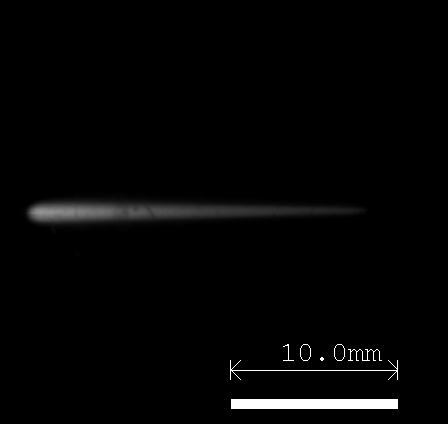
\includegraphics[width=\textwidth]{assets/4 experiments/V1 Spark Ignition Frames/LSP142_SPRK15_Fr130.bmp}
        \caption{\qty{13.0}{ms}}
        %\label{fig:ignition_frames_21}
    \end{subfigure}
    \caption{LSP spark initiation: \qty{3080}{W}, \qty{20}{bar}. \shotsettings{LSP142\_SPRK15}{0.1?? CHANGE}{22}{2048}}
    \label{fig:V1_spark_initiation_frames}
\end{figure}

    \begin{figure}[h]
    \centering
    \begin{subfigure}[t]{0.47\textwidth}
        \centering
        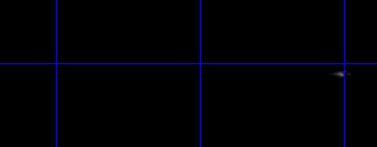
\includegraphics[width=\textwidth]{assets/5 results/1msFrames/16.jpg}
        \caption{\qty{1.6}{ms}}
        \label{fig:growth_frames_16}
    \end{subfigure}
    \hfill
    \begin{subfigure}[t]{0.47\textwidth}
        \centering
        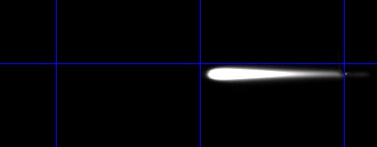
\includegraphics[width=\textwidth]{assets/5 results/1msFrames/26.jpg}
        \caption{\qty{2.6}{ms}}
        \label{fig:growth_frames_26}
    \end{subfigure}
    \hfill
    \begin{subfigure}[t]{0.47\textwidth}
        \centering
        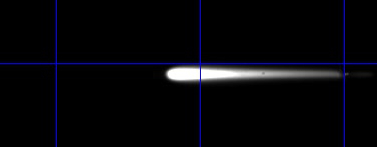
\includegraphics[width=\textwidth]{assets/5 results/1msFrames/36.jpg}
        \caption{\qty{3.6}{ms}}
        \label{fig:growth_frames_36}
    \end{subfigure}
    \hfill
    \begin{subfigure}[t]{0.47\textwidth}
        \centering
        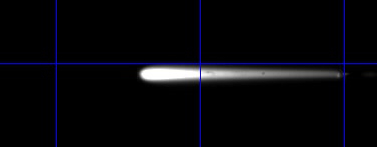
\includegraphics[width=\textwidth]{assets/5 results/1msFrames/46.jpg}
        \caption{\qty{4.6}{ms}}
        \label{fig:growth_frames_46}
    \end{subfigure}
    \hfill
    \begin{subfigure}[t]{0.47\textwidth}
        \centering
        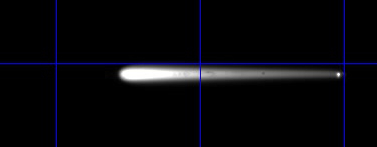
\includegraphics[width=\textwidth]{assets/5 results/1msFrames/56.jpg}
        \caption{\qty{5.6}{ms}}
        \label{fig:growth_frames_56}
    \end{subfigure}
    \hfill
    \begin{subfigure}[t]{0.47\textwidth}
        \centering
        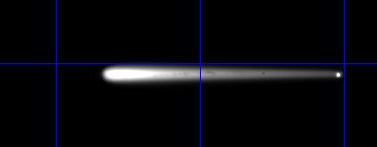
\includegraphics[width=\textwidth]{assets/5 results/1msFrames/66.jpg}
        \caption{\qty{6.6}{ms}}
        \label{fig:growth_frames_66}
    \end{subfigure}
    \hfill
    \begin{subfigure}[t]{0.47\textwidth}
        \centering
        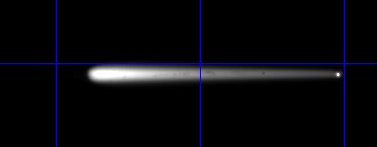
\includegraphics[width=\textwidth]{assets/5 results/1msFrames/76.jpg}
        \caption{\qty{7.6}{ms}}
        \label{fig:growth_frames_76}
    \end{subfigure}
    \hfill
    \begin{subfigure}[t]{0.47\textwidth}
        \centering
        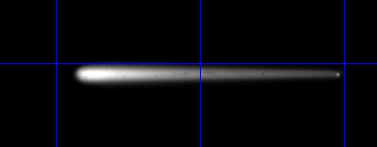
\includegraphics[width=\textwidth]{assets/5 results/1msFrames/86.jpg}
        \caption{\qty{8.6}{ms}}
        \label{fig:growth_frames_86}
    \end{subfigure}
    \hfill
    \begin{subfigure}[t]{0.47\textwidth}
        \centering
        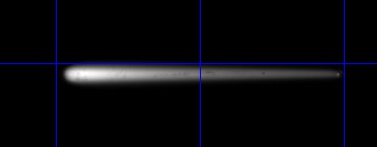
\includegraphics[width=\textwidth]{assets/5 results/1msFrames/96.jpg}
        \caption{\qty{9.6}{ms}}
        \label{fig:growth_frames_96}
    \end{subfigure}
    \hfill
    \begin{subfigure}[t]{0.47\textwidth}
        \centering
        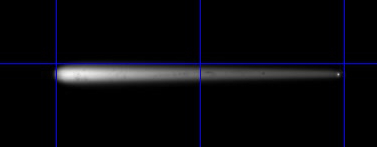
\includegraphics[width=\textwidth]{assets/5 results/1msFrames/106.jpg}
        \caption{\qty{10.6}{ms}}
        \label{fig:growth_frames_106}
    \end{subfigure}
    \hfill
    \begin{subfigure}[t]{0.47\textwidth}
        \centering
        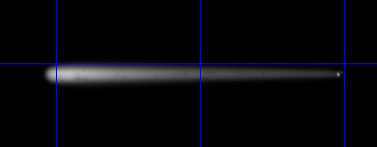
\includegraphics[width=\textwidth]{assets/5 results/1msFrames/116.jpg}
        \caption{\qty{11.6}{ms}}
        \label{fig:growth_frames_116}
    \end{subfigure}
    \caption[LSP growth throughout 10-ms-laser pulse]{LSP growth throughout 10-ms-laser pulse: \qty{3080}{W}, \qty{20.29}{bar}. The blue grid is spaced by \qty{10}{mm}. \shotsettings{LSP1\_PS1}{0.1}{22}{2048}}
    \label{fig:growth_frames}
\end{figure}

    \begin{figure}[h]
        \centering
        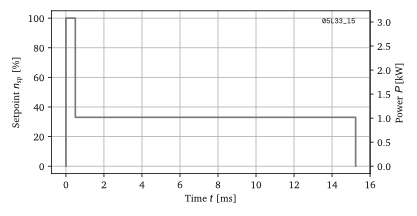
\includegraphics[]{assets/5 results/pulse_profile}
        \caption{Typical stepped-pulse profile: \texttt{05L33\_15}}
        \label{fig:pulse_stepProfile}
    \end{figure}

    \begin{figure}[h]
        \centering
        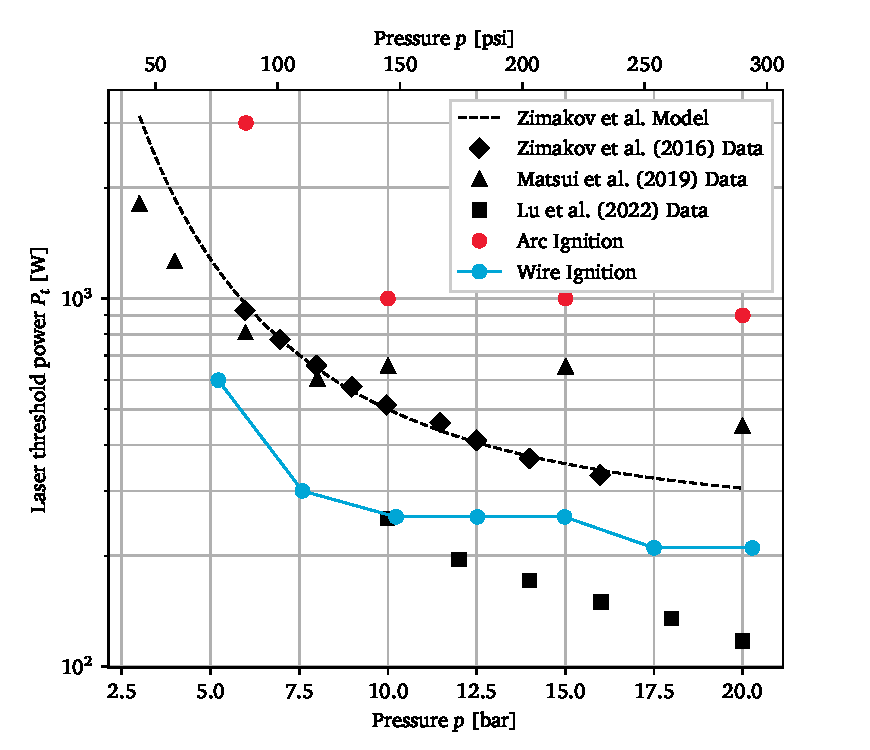
\includegraphics[]{assets/5 results/powerthreshold}
        \caption[Pressure-Power LSP threshold exploration]{Pressure-Power LSP threshold exploration. Experimental data for two different ignition methods is compared to past literature. \textcite{zimakovInteractionNearIRLaser2016}'s model is fitted to wire ignition data as the blue dashed line.}
        \label{fig:powerthreshold}
    \end{figure}

    \section{Heat deposition}

    \begin{figure}[h]
        \centering
        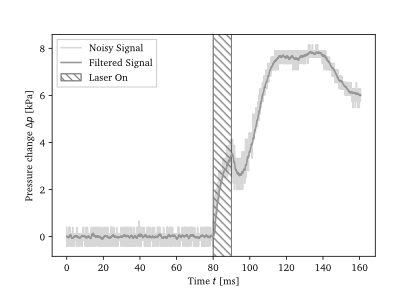
\includegraphics[]{assets/5 results/pressure_noise}
        \caption[Typical pressure change during and after LSP]{Typical pressure change during and after LSP at \qty{3080}{W}, \qty{20.29}{bar}. Both the raw noisy signal and the filtered signal are shown.}
        \label{fig:pressure_noise}
    \end{figure}

    \begin{figure}[h]
        \centering
        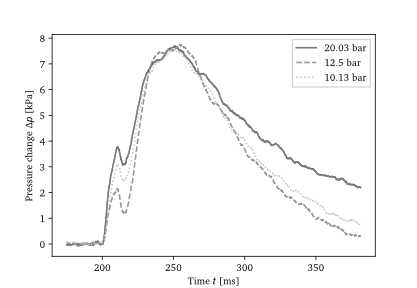
\includegraphics[]{assets/5 results/pressure_pressures}
        \caption{Effect of varying initial pressure on pressure rise resulting from LSP}
        \label{fig:pressure_pressures}
    \end{figure}

    \begin{figure}[h]
        \centering
        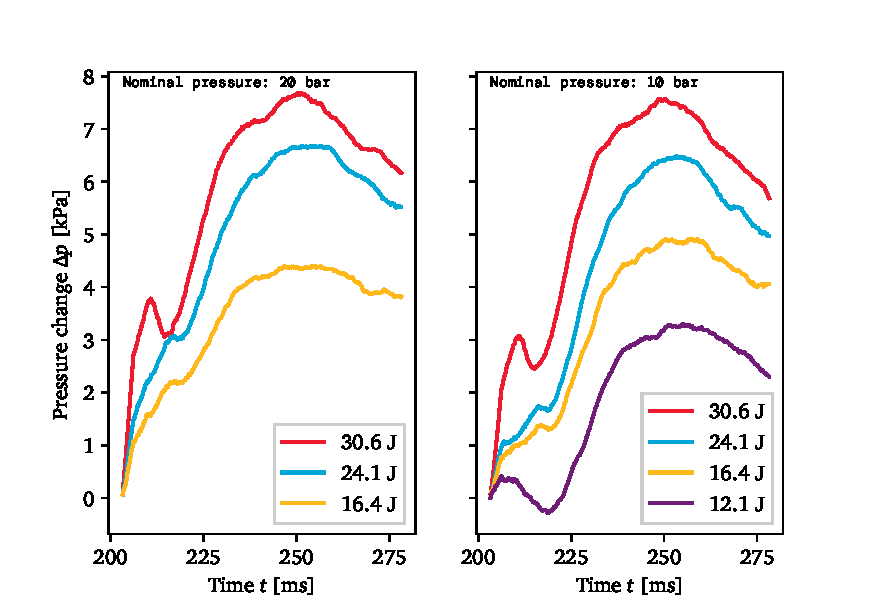
\includegraphics[]{assets/5 results/pressure_powers}
        \caption{Effect of varying the laser pulse energy on the pressure rise resulting from LSP}
        \label{fig:pressure_powers}
    \end{figure}

    \begin{figure}[h]
        \centering
        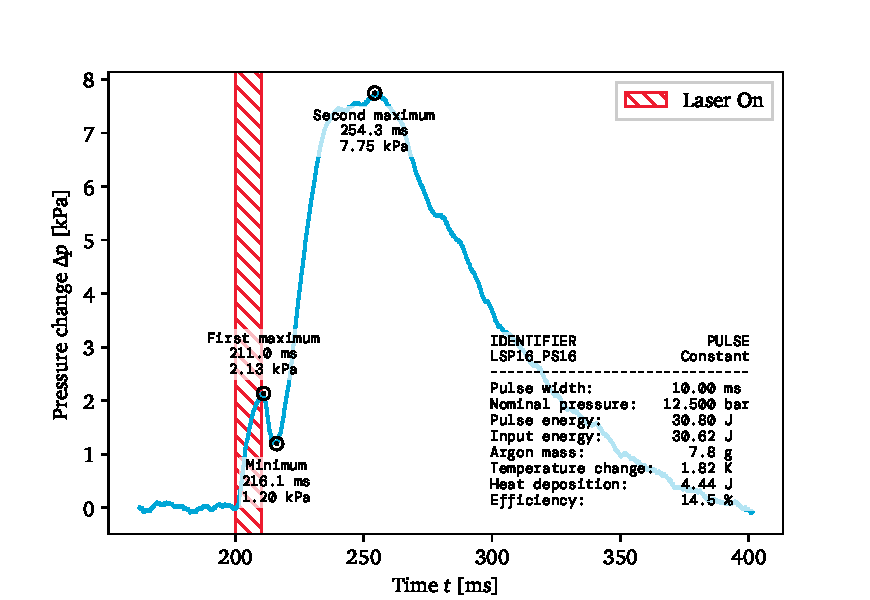
\includegraphics[]{assets/5 results/pressure_an_LSP16_PS16}
        \caption[Detailed analysis of pressure rise profile]{Detailed analysis of pressure rise profile, \qty{3080}{W}, \qty{12.5}{bar}.}
        \label{fig:}
    \end{figure}